\documentclass[12pt]{article}
\usepackage{uswdwms}

% Setup document variables
\def \institutionid{University of South Wales}
\def \unicoursename{Applied Cyber Security}
\def \unimodulecode{IY2D502}
\def \unimodulename{Secure Systems}
\def \unimodulelect{Elaine Haigh}
\title{Portfolio One}
\author{David Sanders}
\def \unistudentid{17135397}
\date{\today}

\makeatletter
\let\thetitle\@title
\let\theauthor\@author
\let\thedate\@date
\makeatother
%

% Setup header and footer
\pagestyle{fancy}
% Create headers and footers with full datetime in regional text style
% \makeheadersandfooters{\scriptsize\scshape \unimodulecode: \thetitle}{\scriptsize \unistudentid}{\footnotesize \DTMnow}{\footnotesize \thepage}

% Create headers and footers with full datetime in ISO style
\makeheadersandfooters{\scriptsize\scshape \unimodulecode: \thetitle}{\scriptsize \unistudentid}{\footnotesize {\DTMsetstyle{iso}\DTMnow}}{\footnotesize \thepage}

% Create headers and footers with full datetime in regional numeric style
% \makeheadersandfooters{\scriptsize\scshape \unimodulecode: \thetitle}{\scriptsize \unistudentid}{\footnotesize {\DTMsetregional[numeric]\DTMnow}}{\footnotesize \thepage}
%

\begin{document}
% \makeuswtitlepage{}
\begin{uswtitlepage}
  \begin{table}[H]
    \centering
    \newcolumntype{v}{>{\centering\arraybackslash}p{7cm}}
    \begin{tabularx}{7cm + 2\tabcolsep + \arrayrulewidth}{v}
      \textsc{David Sanders} \tabularnewline
      \makecell[c{v}]{
        \centering
        \vspace{-\textfloatsep}
        \begin{personcontact}{gh_17135397.png}{0.1}
          \textcolor{light-gray}{\faEnvelope} \href{mailto:17135397@students.southwales.ac.uk}{17135397} \tabularnewline
          \textcolor{light-gray}{\faLinkedin} \href{https://www.linkedin.com/in/dwmsanders/}{dwmsanders} \tabularnewline
          \textcolor{light-gray}{\faGithub} \href{https://github.com/david-wm-sanders}{david-wm-sanders} \tabularnewline
        \end{personcontact}
      } \tabularnewline
    \end{tabularx}
  \end{table}
\end{uswtitlepage}

\tableofcontents

\pagebreak\part{\textsc{Chris Roberts}}
\textcolor{deep-gray}{\textit{Notes to the reader: in order to align the content of this report with that of the presentation given to Chris Roberts, I have chosen to split this report into two parts. The first part of the report is an executive summary which details RFID technologies in access control contexts (the task for which they are most deployed in organisations). It was written with the intent that it should be possible to provide the executive summary as a piece of supplementary material to audiences viewing tangible demonstrations of the threat detailed. The second part of the report is dedicated to exploring the practical, legal, and ethical issues with regard to demonstrating these threats and tools -- it is directed at and written for those performing demonstrations.}}

\section{RFID Access Control Threats}
RFID \textit{(Radio-frequency identification)} technologies, of which NFC \textit{(Near-field communication)} is a specific implementation, allow for wireless \textit{(contactless)} communications between devices \textit{(such as access card readers and mobile phones)} and objects with embedded or attached RFID tags \textit{(such as access cards)}. RFID technologies are being used to carry out tasks such as ID badging, access control, personnel tracking, inventory management, asset tracking, counterfeit prevention, supply chain management, and contactless payment. Although RFID deployments can present considerable advantages from a commercial and financial point of view, they can also introduce new security concerns.\\

\noindent In the context of most businesses, a primary use of RFID is for ID badging and access control \textit{(where the ID badge tag also acts as the access control authenticator)}. Even this limited subset of use cases presents many opportunities for criminal or hostile state actors to attempt to interfere with the intended electronic operation of the RFID system. As RFID access control systems continue to become more widespread and bigger in deployment scale, the attack surface and attraction to hostile actors will continue to increase.\\

\noindent The major threats to such systems are the loss of confidential \textit{(and possibly personal)} information stored on tags to hostile actors by unauthorised tag reading and cloning or spoofing tags by hostile actors \textit{(so that they can conduct malicious actions in restricted areas that require physical access)}.\\

\noindent In order to mitigate these threats, the use of encryption \textit{(provided by RFID/NFC tag architectures and implementations)} can be used to protect information stored on the card and reduce the vulnerability of the tag to cloning and spoofing attacks.\\

\noindent However, it should be noted that it is possible that some organisations, operating large legacy access control systems, may be deploying tags where the encryption system provided was not used. Any personal data stored on those tags \textit{(such as ID numbers)} would then be vulnerable to being stolen by hostile actors, and could possibly be used to track tags \textit{(i.e. people)} in an unauthorised fashion. Such unencrypted tags could also be surreptitiously cloned by hostile actors - sometimes with the relative ease of using an app such as the MIFARE Classic Tool\footnote{\href{https://play.google.com/store/apps/details?id=de.syss.MifareClassicTool&hl=en_GB&rdid=de.syss.MifareClassicTool}{Google Play Store: MIFARE Classic Tool}} which is available on the Google Play Store.\\

\noindent Furthermore, the proprietary encryption scheme deployed with the MIFARE Classic tag family has been compromised since 2008\footnote{\href{http://www.cs.ru.nl/~flaviog/publications/Security_Flaw_in_MIFARE_Classic.pdf}{Schreur, R. et al (2008) \textit{Security Flaw in MIFARE Classic}}} and the hardened MIFARE Classic EV1 tags have been compromised since 2015\footnote{\href{http://cs.ru.nl/~rverdult/Ciphertext-only_Cryptanalysis_on_Hardened_Mifare_Classic_Cards-CCS_2015.pdf}{Meijer, C. and Verdult, R. (2015) \textit{Ciphertext-only Cryptanalysis on Hardened Mifare Classic Cards}}}. These attacks make it possible to clone encrypted MIFARE Classic tags, in a short amount of time, with equipment that is relatively cheap and available to motivated criminal or hostile state actors. The manufacturer, NXP Semiconductors, have officially recommended that MIFARE Classic-based systems are updated to use tags and readers from more secure MIFARE tag families.\footnote{\href{https://www.mifare.net/en/products/chip-card-ics/mifare-classic/frequently-asked-questions/}{MIFARE: FAQs on the security of the MIFARE Classic}} It should be noted, however, that attacks against the MIFARE DESFire\footnote{\href{http://www.proxmark.org/files/Documents/13.56\%20MHz\%20-\%20MIFARE\%20DESFire/Cloning_Cryptographic_RFID_Cards_for_25USD-WISSEC_2010.pdf}{Kasper, T. et al (2016) \textit{Cloning Cryptographic RFID Cards for 25\$}}} and Ultralight\footnote{\href{https://www.youtube.com/watch?v=-uvvVMHnC3c}{YouTube: NFC For Free Rides and Rooms (on your phone)}} families have also been published.\\

\noindent In light of this, it would be prudent to take additional actions to further mitigate the security concerns introduced by RFID ID badge/access control deployments and protect critical organisational assets. The deployment of multiple factor authentication systems \textit{(e.g. a door PIN code and/or biometrics in addition to access cards)} to protect critical assets \textit{(such as server rooms)} could be a robust measure to protect against current and future vulnerabilities in tag implementations. Another mitigative action could be issuing shielded tag carriers or card wallets to users \textit{(to reduce the risk of tag tracking and reads-at-range to steal data from unencrypted or poorly encrypted tags)}.\\

\noindent In conclusion, the current and future risks of RFID access control systems are uncertain. Board members and upper management will have significant stake in decisions taken in the event that a vulnerability is discovered in the access control system deployed in their organisation whether or not the vulnerability is found during a security review/penetration test or as part of a post-incident response analysis. A significant vulnerability in a system could necessitate extensive hardware and infrastructure fixes to rectify. As a result of this, the argument can be made that management should take proactive actions \textit{(such as implementing the mitigative measures detailed above and codifying them in policies)} in order to improve system resilience and guard against future threat. Finally, all RFID ID badge/access control systems should make use of encryption as a baseline.

% \pagebreak
\section{Tangible Demonstration}
Performing a demonstration of these attacks against a live production system would come with numerous legal and ethical issues such as the risk of compromising personal data (if the card tested in the demonstration happens to contain very sensitive personal data) and the risk of violating the terms and conditions surrounding the deployment of the RFID access control system.

Notwithstanding the above, there would also be significant practical issues.
Firstly, the presentation and demonstration could only be performed at venues where permission to test the infrastructure publicly was given, which will not be many. Secondly, some cards (if provided at random by audience members) may be resistant to the variations of attacks vs MIFARE Classic that are being demonstrated. This would result in the demonstration failing; however, the cards may yet be vulnerable to other attacks, such as the DESFire and Ultralight.

With regards to the above, utilising a portable demonstration setup that consists of an access card reader, a cloning device (for example, an Android phone with the MIFARE Classic Tool app installed), an unencrypted MIFARE Classic 4k tag, and a blank UID-writable MIFARE Classic 4k tag would seem to be the optimal solution for providing a consistent demonstration platform. The reader could simply indicate an authentication success (door unlocked) or an authentication failure (door remains locked) with a green and red LED respectively. The process of the demonstration would entail:

\begin{enumerate}
  \item Proving that the card to be cloned to is in fact blank. This would be done by showing that it fails authentication with the access card reader.
  \item Showing that all sectors (some of which could contain example personal data) can be read from unencrypted MIFARE 4k card and dumped to a file on the cloning device (mobile phone) with the MIFARE Classic Tool.
  \item Showing that the dumped image of the original valid card can be cloned to a UID-writable (sector 0 read-write) equivalent tag that implements the MIFARE Classic standard by using the write tag functionality within MIFARE Classic Tool.
  \item Proving that the card cloned to can now be used to authenticate successfully with the access card reader.
\end{enumerate}


\pagebreak\part{\textsc{Sal Scarpato}}
\section{Introduction}
For this assignment, my task was to deploy and secure a LAMP stack. As a solution for deploying web applications and sites, the term `LAMP' originally comes from the components: Linux \textit{(as the deployment operating system)}, Apache \textit{(as the HTTP web server)}, MySQL \textit{(as the database server/management system)}, and PHP \textit{(as the web site/application development language)}.

However, in modern usage, the term "LAMP" refers to a deployment model where alternatives can be used in lieu of the original components.

In seeking to meet the security constraints of the requirements, I endeavoured to choose development and deployment frameworks that would enable me to secure the web application and server as effectively as possible from the start.

As a methodology for building scalable secure applications or software-as-service, I followed the \texttt{Twelve-Factor App}\footnote{\href{https://12factor.net/}{The Twelve Factor App}} suggestions whilst also evaluating additional security risk considerations and pertinent mitigations.

As such, I decided to deploy the MySQL and gunicorn/Flask instances in separate docker containers.

This deployment strategy forces the web application to be written in such as way that it can be bundled into a least-privilege container with all of its dependencies -- being able to spin up web application instances in this manner makes the application scalable whilst also improving security by segregating the different components \textit{(database, server)} from each other in separate containers.

As a reference for learning Flask and understanding how to lay out Flask web applications in a modular fashion so that they can be secured and extended easily, I made extensive use of Miguel Grinberg's Flask Mega-Tutorial\footnote{\href{https://blog.miguelgrinberg.com/post/the-flask-mega-tutorial-part-i-hello-world}{Miguel Grinberg's Flask Mega-Tutorial}}. The wide availability of tutorials and documentation for Python and Flask, as well as significant security discourse, make it a simple and versatile language/framework to develop secure systems with.

\begin{displaytable}{\label{display:lamp_stack}}{Dockerised LAMP Stack}
  \paragraph{\href{http://releases.ubuntu.com/18.10/ubuntu-18.10-live-server-amd64.iso}{\faUbuntu\ Ubuntu Server 18.10}}
  \hspace{-0.6em}-- as the deployment operating system.
  \paragraph{\href{https://hub.docker.com/\_/mysql}{\faDatabase\ MySQL}}
  \hspace{-0.6em}-- as the database server/management system, running in a docker container and only exposed to other containers explicitly by linking
  \paragraph{\href{https://pypi.org/project/gunicorn/}{\faServer\ Gunicorn}}
  \hspace{-0.6em}-- as the WSGI HTTP Server, running the web application in a custom built container based on the python3.7-slim docker image.
  \paragraph{\href{https://pypi.org/project/Flask/1.0.2/}{\faPython\ Flask}}
  \hspace{-0.6em}-- as the web application development framework, with Python3 and jinja as the development languages.
  \vspace{1em}
\end{displaytable}


\pagebreak
\section{Deployment Methodology}
Underlined is a basic methodology for deploying the server, MySQL, and the web application with gunicorn.

\begin{enumerate}[leftmargin=0em,label=\protect\listlabelcircle{\arabic*}]
  \item Set up Ubuntu Server 18.10 \footnote{\href{http://releases.ubuntu.com/18.10/ubuntu-18.10-live-server-amd64.iso}{\texttt{ubuntu-18.10-live-server-amd64.iso}}} using the Subiquity\footnote{\href{https://github.com/CanonicalLtd/subiquity}{\faGithub\ CanonicalLtd/subiquity}} installer
    \begin{enumerate}[label=\Roman*~\textcolor{light-gray}{|}]
      \item Select \textit{Install Ubuntu Server} at the GRUB2 boot menu\\
      \textcolor{deep-gray}{\textit{[Figure~\ref{fig:IY2D502-2019-02-21-19-15-19}]}}
      \item For standard UK keyboards, set the layout and variant to \textit{English {UK}} and \textit{English (UK, extended, with Win keys)} respectively -- this will help to ensure that passwords are entered correctly\\
      \textcolor{deep-gray}{\textit{[Figure~\ref{fig:IY2D502-2019-02-21-19-16-03}]}}
      \item Select \textit{Install Ubuntu} for a normal server deployment\\
      \textcolor{deep-gray}{\textit{[Figure~\ref{fig:IY2D502-2019-02-21-19-16-06}]}}
      \item Choose to set up Logical Volume Management \textit{(LVM)} when prompted to configure filesystem setup\\
      \textcolor{deep-gray}{\textit{[Figure~\ref{fig:IY2D502-2019-02-21-19-16-38}]}}
      \item Confirm the default LVM filesystem configuration provided by the installer -- in order to increase security it would be possible, at this stage, to set up LVM with LUKS\footnote{\href{https://gitlab.com/cryptsetup/cryptsetup/}{\faGitlab\ cryptsetup/cryptsetup/}} full-disk-encryption and configure separate partitions for \texttt{/tmp} and \texttt{/var} so that they could have size limitations and be mounted with options like \term{noexec} \textit{(to prevent the executable of binaries on a partition where user uploaded data is stored)}\\
      \textcolor{deep-gray}{\textit{[Figure~\ref{fig:IY2D502-2019-02-21-19-16-43}]}}
      \item Configure the server by providing a name, server name \textit{(hostname)}, username, password -- it is also possible to import SSH identities from GitHub, as exhibited in the screenshot, and thus configure immediate secure access over SSH with public-private key authentication\\
      \textcolor{deep-gray}{\textit{[Figure~\ref{fig:IY2D502-2019-02-21-19-17-27}]}}
      \item Review and choose snaps for install \textit{(this allows the server to be quickly provisioned)} -- select nothing here as Docker will be installed manually later in this methodology\\
      \textcolor{deep-gray}{\textit{[Figure~\ref{fig:IY2D502-2019-02-21-19-17-58}]}}
      \item Reboot when prompted to finish the installation
      \item Upon logging into the new server install, check for updates and upgrade if required -- on Ubuntu, this is done with \texttt{apt} using the commands:
        \begin{itemize}
          \item \term{sudo apt update}
          \item \term{sudo apt upgrade}
        \end{itemize}
      \textcolor{deep-gray}{\textit{[Figure~\ref{fig:IY2D502-2019-02-21-19-22-44}]}}
    \end{enumerate}
  \pagebreak
  \item Download latest \texttt{salapp}
    \begin{enumerate}[label=\Roman*~\textcolor{light-gray}{|}]
      \item Clone \texttt{salapp} from \href{https://github.com/david-wm-sanders/uswacs-2-iy2d502-salapp}{\faGithub\ david-wm-sanders/uswacs-2-iy2d502-salapp} using:\\
      \term{git clone git@github.com:david-wm-sanders/uswacs-2-iy2d502-salapp.git}
    \end{enumerate}
  \item Install \texttt{docker-ce}\footnote{\href{https://github.com/docker/docker-ce}{\faGithub\ docker/docker-ce}} \textit{(Docker Community Edition)}
    \begin{enumerate}[label=\Roman*~\textcolor{light-gray}{|}]
      \item Use \term{sudo apt install docker.io} to install \texttt{docker} on the server\\
      \textcolor{deep-gray}{\textit{[Figure~\ref{fig:IY2D502-2019-02-21-23-29-41}]}}
    \end{enumerate}
  \item Set up a containerised MySQL instance using docker
    \begin{enumerate}[label=\Roman*~\textcolor{light-gray}{|}]
      \item To start a MySQL container for the first time, run the \texttt{salapp/start\_mysql.sh} script \textit{(shown in Listing~\ref{lst:meth:start_mysql_sh})} with \term{sudo ./start\_mysql.sh}\\
        This script will \term{run} a docker container:
        \begin{itemize}
          \item \term{--name mysql}: named \texttt{mysql}
          \item \term{-d}: detached so that it runs in the background
          \item \term{-e}: with environment variables to configure a random root password, create a database for the web application, and create a user with a password for the web application
          \item from the \texttt{mysql/mysql-server:latest}\footnote{\href{https://hub.docker.com/\_/mysql}{Docker Hub: MySQL}} image on Docker Hub\footnote{\href{https://docs.docker.com/docker-hub/repos/}{Docker Docs: Docker Hub Repositories}}
        \end{itemize}
        \begin{listing}[H]
          \captionsetup{skip=\skiplistingcaptionlen}
          \inputminted[breakanywhere]{bash}{../uswacs-2-iy2d502-salapp/start_mysql.sh}
          \caption{\texttt{salapp/start\_mysql.sh}}
          \label{lst:meth:start_mysql_sh}
        \end{listing}
    \end{enumerate}
  \pagebreak
  \item Deploy \texttt{salapp} with docker
    \begin{enumerate}[label=\Roman*~\textcolor{light-gray}{|}]
      \item To build the \texttt{salapp} container from the \texttt{Dockerfile}, run the \texttt{salapp/make\_salapp.sh} script \textit{(shown in Listing~\ref{lst:meth:make_salapp_sh})} with \term{sudo ./make\_salapp.sh}\\
        This process entails:
        \begin{itemize}
          \item Using \texttt{docker build} to create a new container, tagged with \term{-t salapp:latest}, from the \texttt{Dockerfile} in \term{.}
          \item Having a \texttt{Dockerfile} \textit{(shown in Listing~\ref{lst:meth:Dockerfile})} that defines commands that:
            % \begin{enumerate}[label=\textcolor{light-gray}{\roman*\~}]
            \begin{enumerate}[label=\textcolor{deep-gray}{\roman*\textasciitilde}]
              \item Derive the new container \term{FROM} the \texttt{python:3.7-alpine} image
              \item \term{adduser} called \texttt{salapp} with a home directory
              \item Set the \term{WORKDIR} in the container to the home directory for the \texttt{salapp} user
              \item \term{COPY} \texttt{salapp/requirements.txt} \textit{(shown in \hyperref[fcl:salapp:requirements]{requirements.txt})} into the container
              \item \term{RUN python -m venv venv} in order to create a virtual environment called \texttt{venv}
              \item \term{RUN  venv/bin/pip install -r requirements.txt} in order to install the dependencies in the \texttt{venv}
              \item \term{RUN venv/bin/pip install gunicorn pymysql} in order to install \texttt{gunicorn} \textit{(a WSGI HTTP server)} and python library \texttt{pymysql} in the \texttt{venv}
              \item \term{COPY} in the \texttt{salapp/app} and \texttt{salapp/migrations} directories
              \item \term{COPY} in the \texttt{salapp/salapp.py} and \texttt{boot.sh} files
              \item Make \texttt{boot.sh} executable with \term{RUN chmod a+x boot.sh}
              \item Use \term{ENV} to set environment variables inside the container
              \item Change ownership of the directories to the \texttt{salapp} user with \term{chown}
              \item Become \term{USER salapp} for all commands after this and each time the container is started
              \item \term{EXPOSE} ports externally to the container
              \item Make \texttt{salapp/boot.sh} the \term{ENTRYPOINT} of the container
            \end{enumerate}
          \item Having a \texttt{boot.sh} \textit{(show in Listing~\ref{lst:meth:boot_sh})} that defines how the container starts -- in this case:
            \begin{enumerate}[label=\textcolor{deep-gray}{\roman*\textasciitilde}]
              \item Activating the virtual environment \textit{(which will add the path to ./venv/bin/ to the PATH)}
              \item Running \term{flash db upgrade} to perform any initial table creation or existing database version migrations
              \item Executing \texttt{gunicorn} with:
                \begin{itemize}
                  \item \term{-b :5000}: to bind the server to port 5000
                  \item \term{--access-logfile - --error-logfile -}: to write access and error logfiles to standard output so docker can log it
                  \item \term{salapp:app}: to set the Flask app instance in salapp as the logic
                \end{itemize}
            \end{enumerate}
        \end{itemize}
        \begin{listing}[H]
          \captionsetup{skip=\skiplistingcaptionlen}
          \inputminted[breakanywhere]{bash}{../uswacs-2-iy2d502-salapp/make_salapp.sh}
          \caption{\texttt{salapp/make\_salapp.sh}}
          \label{lst:meth:make_salapp_sh}
        \end{listing}
        \begin{listing}[H]
          \captionsetup{skip=\skiplistingcaptionlen}
          \inputminted[breakanywhere]{bash}{../uswacs-2-iy2d502-salapp/boot.sh}
          \caption{\texttt{salapp/boot.sh}}
          \label{lst:meth:boot_sh}
        \end{listing}
        \begin{listing}[H]
          \captionsetup{skip=\skiplistingcaptionlen}
          \inputminted[breakanywhere]{bash}{../uswacs-2-iy2d502-salapp/Dockerfile}
          \caption{\texttt{salapp/Dockerfile}}
          \label{lst:meth:Dockerfile}
        \end{listing}
      \item start salapp with \term{./start\_salapp.sh} \todo{include listings here}
    \end{enumerate}
  \pagebreak
  \item \todo{Connect to web application and trigger shit}
  \item \todo{Show how \texttt{mysql\_root\_login.sh} and \texttt{mysql\_salapp\_login.sh} can be used to check that the quotes were entered into the db correctly}
  \item \todo{Create a script to view the security alert logs and demonstrate with evidence}
\end{enumerate}


\pagebreak
\section{Hardening}
\todo{Hardening intro...}

% \pagebreak
\subsection{Ubuntu 18.10 Server: \texttt{salsrv}}
\todo{some text here pls}
% \subsubsection*{Logical Volume Management}
% \paragraph{Partitioning}
% As discussed in the methodology, and although beyond the scope of this report, it would be possible to use Logical Volume Management to define a more resilient partitioning scheme on disk.
%
% This could include having separate paritions for \texttt{/tmp} and \texttt{/var}. In the case of \texttt{/tmp}, benefit would be gained by mounting the drive with \texttt{noexec} if the server was storing user uploaded data in the \texttt{/tmp} partition.
%
% Having separate partitions also increases the resilience of the system by preventing logs, written to \texttt{/var/log} for example, from filing the drive completely and disrupting the operation of the \texttt{/} partition. An attacker could attempt to trigger events that cause logs to be written in order to fill server drives and cause a Denial-of-Service.
%
% In light of this, the use of more finessed partitioning schemes can help to ensure that the integrity and availability of data and the server itself is maintained.
%
% \paragraph{Encryption}
% Fully encrypting drives with LUKS would improve confidentiality significantly
% \subsubsection{User Accounts}
% Locking them down more?
\subsubsection{Locking down SSH via \texttt{/etc/ssh/sshd\_config}}
% https://medium.com/@jasonrigden/hardening-ssh-1bcb99cd4cef
% https://linux-audit.com/audit-and-harden-your-ssh-configuration/
% https://www.cyberciti.biz/tips/linux-unix-bsd-openssh-server-best-practices.html
% https://github.com/BetterCrypto/Applied-Crypto-Hardening/blob/master/src/configuration/SSH/OpenSSH/6.6/sshd_config
% https://gist.github.com/tribou/fcda8e6066776c9eaa47 (with added TORHS goodies...)
% https://security.stackexchange.com/questions/179114/what-are-the-toughest-ssh-daemon-settings-in-terms-of-encryption-handshake-or
% https://security.stackexchange.com/questions/154076/hardening-ssh-security-on-a-debian-9-server
% https://infosec.mozilla.org/guidelines/openssh (taking it to the next level!)

In order to prevent unauthorised remote access via SSH to the server, several steps should be taken to improve the security of the SSH server configuration. This will increase the confidentiality of data on the server \textit{(by further restricting access to the server)} whilst also maintaining integrity and availability for authenticated users.

An element of improving the SSH configuration was performed during the installation by importing SSH identities from GitHub. This allows the user who controls the private keys of those identities to connect to the server out-of-the-gate with public-private key authentication rather than password authentication for SSH connections.

Further harden the SSH server by modifying the configuration in \texttt{/etc/ssh/sshd\_config} \textit{(as shown in Figure~\ref{fig:IY2D502-2019-02-26-17-44-30})}. This involves:
\begin{itemize}
  \item Preventing remote login over SSH to the \texttt{root} account by setting:\\
    \term{PermitRootLogin no}
  \item Setting \term{PasswordAuthentication no} to prevent password authentication for all incoming SSH connections to all accounts completely -- this can be done without worry if the \texttt{authorized\_keys} imported from GitHub during the installation work successfully
\end{itemize}

\subsubsection{Setting up a Firewall}
\label{sec:hardening:firewall}
A firewall can be used to drop all traffic to ports not explicitly allowed to receive incoming traffic -- this effectively closes the port to the outside world.

On Ubuntu, firewall configuration can be performed with the \texttt{ufw} tool \textit{(as shown in Figure~\ref{fig:IY2D502-2019-02-26-19-28-12})}.

This involves:
\begin{itemize}
  \item Starting the firewall with \term{sudo ufw enable}
  \item Adding allow rules with:
    \begin{itemize}
      \item \term{sudo ufw allow ssh}: will allow inbound traffic on port 22
      \item \term{sudo ufw allow http}: will allow inbound traffic on port 80
      \item \term{sudo ufw allow https}: will allow inbound traffic on port 443
    \end{itemize}
  \item Checking that the firewall is active and configured correctly using:\\
    \term{sudo ufw status}
\end{itemize}

\subsubsection{Ensuring that the system in upgraded}
Ensure that the server is patched regularly \textit{(as shown in Figures~\ref{fig:IY2D502-2019-02-22-23-41-29}~and~\ref{fig:IY2D502-2019-02-22-23-44-52})}. Security vulnerabilities in system packages could expose the server to exploits that compromise confidentiality, integrity, and/or availability.

During upgrading it is possible to ascertain the changes \textit{(some of which will be fixes for security vulnerabilities)} made to the packages. For example, in Figure~\ref{fig:IY2D502-2019-02-22-23-44-52}, we can see that \texttt{bind9} was upgraded to version \texttt{1:9.11.4+dfsg-3ubuntu5.1}. Changelogs for Ubuntu packages are published on Launchpad and the changelog for \texttt{bind9} at this version at:\\
\href{https://launchpad.net/ubuntu/+source/bind9/1:9.11.4+dfsg-3ubuntu5.1}{\texttt{https://launchpad.net/ubuntu/+source/<package>/<version}}.

In this changelog, we can see that several security fixes were made by patching the source code for \texttt{bind9}.

In a production environment, a crontab job could be developed to check for updates daily and alert the server administrator(s) when there are security updates.
% \subsubsection*{Anti-Malware: \texttt{rkhunter?}}

\pagebreak
\subsection{Flask application: \texttt{salapp}}
In developing my web application, I endeavoured to embed security and hardening from the start.

I chose to use Python3 as the development language due to my existing familiarity with the language and Flask as the framework because it is lightweight and mature with a significant ecosystem of existing Flask extensions that enhance security by adding CSRF to forms, allowing the definition of custom validators for form inputs, setting security headers, enforcing HTTPS, and so on.

Although I had not used Flask before, I was able to pick it up relatively quickly and integrate security considerations into the web application design from the beginning.

\subsubsection{SQL Injection}
\todo{talk a bit about \^ and the implications it has for C, I, and A}

The \texttt{Flask\_SQLAlchemy} extension is used to use to provide a link between the \texttt{SQLAlchemy} Python library and the Flask web application. If the Object Relational Mapper, provided by \texttt{SQLAlchemy}, is used correctly it is possible to correctly escape all inputs for the database and prevent SQL Injection attacks -- in short, this entails always use the ORM primitives and never directly formulating a SQL query.

The \texttt{quotes} table, and columns therein, are defined in Python in \texttt{salapp/app/models.py} \textit{(shown in Listing~\ref{lst:hard:salapp:app:models.py})}. It is possible here to set constraints on fields in the table, such as the length for the \texttt{db.String} type.

This model definition will be used by \texttt{SQLAlchemy} to interact with the database and can even be used to create the SQL query statements to create new tables that store the fields defined in the model in a database.
\begin{listing}[H]
  \captionsetup{skip=\skiplistingcaptionlen}
  \inputminted[breakanywhere,firstline=5]{python3}{../uswacs-2-iy2d502-salapp/app/models.py}
  \caption{\texttt{salapp/app/models.py}}
  \label{lst:hard:salapp:app:models.py}
\end{listing}

\subsubsection{User Input Validation}
When taking data from clients via the quotes form, it is important to validate the input to ensure that it meets requirements and does not exceed constraints before inserting it in the database. The form definition and validation logic is handled in \hyperref[fcl:uswacs-2-iy2d502-salapp:forms.py]{\texttt{salapp/app/forms.py}}.

The form is defined using the \texttt{Flask-WTF} extension -- this allows us to define the form as a Python class, which is then used to generate the form's HTML code dynamically.

\texttt{Flask-WTF} provides some standard validators, such as \texttt{DataRequired()}, that can be used to validate field input but, more importantly, allows custom validation functions to be defined and used.

Listing~\ref{lst:hard:salapp:app:forms.py:ModelLengthValidator} shows a custom validator that I defined which will, if it exists, acquire the length of the model field passed to it at initialisation and then use this to validate that the field data provided to the server via the form does not exceed the maximum string length for that database column. This validator is also capable of validating that an input has a minimum length.

Listing~\ref{lst:hard:salapp:app:forms.py:SqlInjectionValidator} shows another custom validator that I defined to check if the field data contains possible SQL query terms that could be part of an SQL injection attack attempt. By default, this validator will raise a \texttt{ValidationError} with a message that can be returned to the user's browser so that they can remedy the issue and request a quote successfully. However, it can be set to only log the issue and not reject the data with a \texttt{ValidationError}. This is possible because any SQL terms that bypass this validator will be correctly escaped by \texttt{SQLAlchemy} before they reach the database. The validator will always log a \texttt{SECURITY ALERT} warning, noting that a possible SQL injection attack attempt has occurred. As the \texttt{gunicorn} server running the application is started in such a way as to order access and error logs to be output to the standard output, the security alert warnings will be visible via \term{docker logs} and could be monitored in an automated fashion in a SOC setup.

As a note here, the form fields are defined using a custom subclass of \texttt{StringField} called \texttt{ModelStringField}. This class allows the model field to be passed at initialisation and will use this to set the \texttt{maxlength} attribute for the \texttt{input} tag in the generated HTML. This allows client-side validators to hint to the user that the data they have input will fail validation before they make a request. This is a nicety and provides no additional security to the server as a directive in HTML to perform client-side validation can be ignored by the client.

\begin{listing}[H]
  \captionsetup{skip=\skiplistingcaptionlen}
  \inputminted[breakanywhere,firstline=13,lastline=31]{python3}{../uswacs-2-iy2d502-salapp/app/forms.py}
  \caption{\texttt{salapp/app/forms.py:ModelLengthValidator}}
  \label{lst:hard:salapp:app:forms.py:ModelLengthValidator}
\end{listing}

\begin{listing}[H]
  \captionsetup{skip=\skiplistingcaptionlen}
  \inputminted[breakanywhere,firstline=49,lastline=68]{python3}{../uswacs-2-iy2d502-salapp/app/forms.py}
  \caption{\texttt{salapp/app/forms.py:SqlInjectionValidator}}
  \label{lst:hard:salapp:app:forms.py:SqlInjectionValidator}
\end{listing}

\subsubsection{Cross-Site Request Forgery Protection}
The \texttt{FlaskForm} class that the \texttt{QuoteForm} subclasses in \hyperref[fcl:uswacs-2-iy2d502-salapp:forms.py]{\texttt{salapp/app/forms.py}} can automatically provide and validate a CSRF Protection Token for the form, as long as the\\
\term{\{\{ form.hidden\_tag() \}\}} is included in the form template \textit{(as shown on line 4 of Listing~\ref{lst:hard:salapp:app:templates:get_quote.html:QuoteFormTagExtract})}.

\begin{listing}[H]
  \captionsetup{skip=\skiplistingcaptionlen}
  \begin{minted}[breakanywhere]{html+jinja}
    <!-- DEBUG: include novalidate for the purpose of testing server-side validation -->
        <form action="" method="POST" novalidate>
          <!-- Security considerations: Include the form's hidden tags to enable the CSRF protection by including the token in a hidden field -->
          {{ form.hidden_tag() }}
          <div class="form-row">
            <div class="form-group col-md-6">{{ form.forename(class_='form-control', placeholder=form.forename.label.text) }}</div>
            <div class="form-group col-md-6">{{ form.surname(class_='form-control', placeholder=form.surname.label.text) }}</div>
          </div>
  \end{minted}
  \caption{\texttt{salapp/app/templates/get\_quote.html:QuoteFormTagExtract}}
  \label{lst:hard:salapp:app:templates:get_quote.html:QuoteFormTagExtract}
\end{listing}

\subsubsection{\todo{Adding SSL certs n' ting}}
\todo{add cert for server and integrate in app, then doc}
\subsubsection{\todo{Flask Talisman}}
\todo{integrate in app, then doc what it provides for us}


\pagebreak
\section{Ubuntu 18.10 Server}
\subsection{Why Ubuntu over CentOS?}
\todo{need to drop some of the good shit here - Ubuntu is more maintained? more tutorials exist for debian/ubuntu? better support for newer techs like containers/k8s with microk8s? etc!}
\section{Apache/nginx+gunicorn}
\todo{which one is easier to use? more secure? if containerised, does the load balancer nginx go in a different container from the gunicorn instances running the flask app?}
\section{MySQL}
\todo{ideally in a container if simple af with ubuntu 18.10 and microk8s...}
\section{Flask Web Application}
\subsection{Good reasons to choose Flask/python3 over PHP!}
\subsection{App Code Structure Overview}
\subsection{Secure Web Development}


% APPENDICES
\pagebreak
\appendix
% Insert auto-generated code listing appendix for salapp
% DEBUG: comment for quicker compile while writing rest of report... :/
% \section{Full Code Listings: \texttt{uswacs-2-iy2d502-salapp}}
\subsection{\texttt{.flaskenv}}
\begin{codelisting}
\label{fcl:uswacs-2-iy2d502-salapp:.flaskenv}
\inputminted[breakanywhere]{text}{../uswacs-2-iy2d502-salapp/.flaskenv}\end{codelisting}
\subsection{\texttt{.gitignore}}
\begin{codelisting}
\label{fcl:uswacs-2-iy2d502-salapp:.gitignore}
\inputminted[breakanywhere]{text}{../uswacs-2-iy2d502-salapp/.gitignore}\end{codelisting}
\subsection{\texttt{Dockerfile}}
\begin{codelisting}
\label{fcl:uswacs-2-iy2d502-salapp:Dockerfile}
\inputminted[breakanywhere]{text}{../uswacs-2-iy2d502-salapp/Dockerfile}\end{codelisting}
\subsection{\texttt{boot.sh}}
\begin{codelisting}
\label{fcl:uswacs-2-iy2d502-salapp:boot.sh}
\inputminted[breakanywhere]{bash}{../uswacs-2-iy2d502-salapp/boot.sh}\end{codelisting}
\subsection{\texttt{list\_reqs\_in\_salapp\_venv.sh}}
\begin{codelisting}
\label{fcl:uswacs-2-iy2d502-salapp:list_reqs_in_salapp_venv.sh}
\inputminted[breakanywhere]{bash}{../uswacs-2-iy2d502-salapp/list_reqs_in_salapp_venv.sh}\end{codelisting}
\subsection{\texttt{make\_salapp.sh}}
\begin{codelisting}
\label{fcl:uswacs-2-iy2d502-salapp:make_salapp.sh}
\inputminted[breakanywhere]{bash}{../uswacs-2-iy2d502-salapp/make_salapp.sh}\end{codelisting}
\subsection{\texttt{mysql\_root\_login.sh}}
\begin{codelisting}
\label{fcl:uswacs-2-iy2d502-salapp:mysql_root_login.sh}
\inputminted[breakanywhere]{bash}{../uswacs-2-iy2d502-salapp/mysql_root_login.sh}\end{codelisting}
\subsection{\texttt{mysql\_salapp\_login.sh}}
\begin{codelisting}
\label{fcl:uswacs-2-iy2d502-salapp:mysql_salapp_login.sh}
\inputminted[breakanywhere]{bash}{../uswacs-2-iy2d502-salapp/mysql_salapp_login.sh}\end{codelisting}
\subsection{\texttt{pystyleproj.py}}
\begin{codelisting}
\label{fcl:uswacs-2-iy2d502-salapp:pystyleproj.py}
\inputminted[breakanywhere]{python3}{../uswacs-2-iy2d502-salapp/pystyleproj.py}\end{codelisting}
\subsection{\texttt{requirements.txt}}
\begin{codelisting}
\label{fcl:uswacs-2-iy2d502-salapp:requirements.txt}
\inputminted[breakanywhere]{text}{../uswacs-2-iy2d502-salapp/requirements.txt}\end{codelisting}
\subsection{\texttt{restart\_mysql.sh}}
\begin{codelisting}
\label{fcl:uswacs-2-iy2d502-salapp:restart_mysql.sh}
\inputminted[breakanywhere]{bash}{../uswacs-2-iy2d502-salapp/restart_mysql.sh}\end{codelisting}
\subsection{\texttt{salapp.py}}
\begin{codelisting}
\label{fcl:uswacs-2-iy2d502-salapp:salapp.py}
\inputminted[breakanywhere]{python3}{../uswacs-2-iy2d502-salapp/salapp.py}\end{codelisting}
\subsection{\texttt{show\_salapp\_logs.sh}}
\begin{codelisting}
\label{fcl:uswacs-2-iy2d502-salapp:show_salapp_logs.sh}
\inputminted[breakanywhere]{bash}{../uswacs-2-iy2d502-salapp/show_salapp_logs.sh}\end{codelisting}
\subsection{\texttt{start\_mysql.sh}}
\begin{codelisting}
\label{fcl:uswacs-2-iy2d502-salapp:start_mysql.sh}
\inputminted[breakanywhere]{bash}{../uswacs-2-iy2d502-salapp/start_mysql.sh}\end{codelisting}
\subsection{\texttt{start\_salapp.sh}}
\begin{codelisting}
\label{fcl:uswacs-2-iy2d502-salapp:start_salapp.sh}
\inputminted[breakanywhere]{bash}{../uswacs-2-iy2d502-salapp/start_salapp.sh}\end{codelisting}
\subsection{\texttt{tox.ini}}
\begin{codelisting}
\label{fcl:uswacs-2-iy2d502-salapp:tox.ini}
\inputminted[breakanywhere]{text}{../uswacs-2-iy2d502-salapp/tox.ini}\end{codelisting}
\subsection{\texttt{app/\_\_init\_\_.py}}
\begin{codelisting}
\label{fcl:uswacs-2-iy2d502-salapp:__init__.py}
\inputminted[breakanywhere]{python3}{../uswacs-2-iy2d502-salapp/app/__init__.py}\end{codelisting}
\subsection{\texttt{app/config.py}}
\begin{codelisting}
\label{fcl:uswacs-2-iy2d502-salapp:config.py}
\inputminted[breakanywhere]{python3}{../uswacs-2-iy2d502-salapp/app/config.py}\end{codelisting}
\subsection{\texttt{app/errors.py}}
\begin{codelisting}
\label{fcl:uswacs-2-iy2d502-salapp:errors.py}
\inputminted[breakanywhere]{python3}{../uswacs-2-iy2d502-salapp/app/errors.py}\end{codelisting}
\subsection{\texttt{app/forms.py}}
\begin{codelisting}
\label{fcl:uswacs-2-iy2d502-salapp:forms.py}
\inputminted[breakanywhere]{python3}{../uswacs-2-iy2d502-salapp/app/forms.py}\end{codelisting}
\subsection{\texttt{app/models.py}}
\begin{codelisting}
\label{fcl:uswacs-2-iy2d502-salapp:models.py}
\inputminted[breakanywhere]{python3}{../uswacs-2-iy2d502-salapp/app/models.py}\end{codelisting}
\subsection{\texttt{app/routes.py}}
\begin{codelisting}
\label{fcl:uswacs-2-iy2d502-salapp:routes.py}
\inputminted[breakanywhere]{python3}{../uswacs-2-iy2d502-salapp/app/routes.py}\end{codelisting}
\subsection{\texttt{app/templates/200.html}}
\begin{codelisting}
\label{fcl:uswacs-2-iy2d502-salapp:200.html}
\inputminted[breakanywhere]{html+jinja}{../uswacs-2-iy2d502-salapp/app/templates/200.html}\end{codelisting}
\subsection{\texttt{app/templates/404.html}}
\begin{codelisting}
\label{fcl:uswacs-2-iy2d502-salapp:404.html}
\inputminted[breakanywhere]{html+jinja}{../uswacs-2-iy2d502-salapp/app/templates/404.html}\end{codelisting}
\subsection{\texttt{app/templates/410.html}}
\begin{codelisting}
\label{fcl:uswacs-2-iy2d502-salapp:410.html}
\inputminted[breakanywhere]{html+jinja}{../uswacs-2-iy2d502-salapp/app/templates/410.html}\end{codelisting}
\subsection{\texttt{app/templates/500.html}}
\begin{codelisting}
\label{fcl:uswacs-2-iy2d502-salapp:500.html}
\inputminted[breakanywhere]{html+jinja}{../uswacs-2-iy2d502-salapp/app/templates/500.html}\end{codelisting}
\subsection{\texttt{app/templates/\_site.html}}
\begin{codelisting}
\label{fcl:uswacs-2-iy2d502-salapp:_site.html}
\inputminted[breakanywhere]{html+jinja}{../uswacs-2-iy2d502-salapp/app/templates/_site.html}\end{codelisting}
\subsection{\texttt{app/templates/about.html}}
\begin{codelisting}
\label{fcl:uswacs-2-iy2d502-salapp:about.html}
\inputminted[breakanywhere]{html+jinja}{../uswacs-2-iy2d502-salapp/app/templates/about.html}\end{codelisting}
\subsection{\texttt{app/templates/get\_quote.html}}
\begin{codelisting}
\label{fcl:uswacs-2-iy2d502-salapp:get_quote.html}
\inputminted[breakanywhere]{html+jinja}{../uswacs-2-iy2d502-salapp/app/templates/get_quote.html}\end{codelisting}
\subsection{\texttt{app/templates/index.html}}
\begin{codelisting}
\label{fcl:uswacs-2-iy2d502-salapp:index.html}
\inputminted[breakanywhere]{html+jinja}{../uswacs-2-iy2d502-salapp/app/templates/index.html}\end{codelisting}

% Insert evidential screenshots appendix
\section{Evidential Screenshots}
\begin{figure}[h!]
\centering
\captionsetup{skip=\skipfigurecaptionlen}
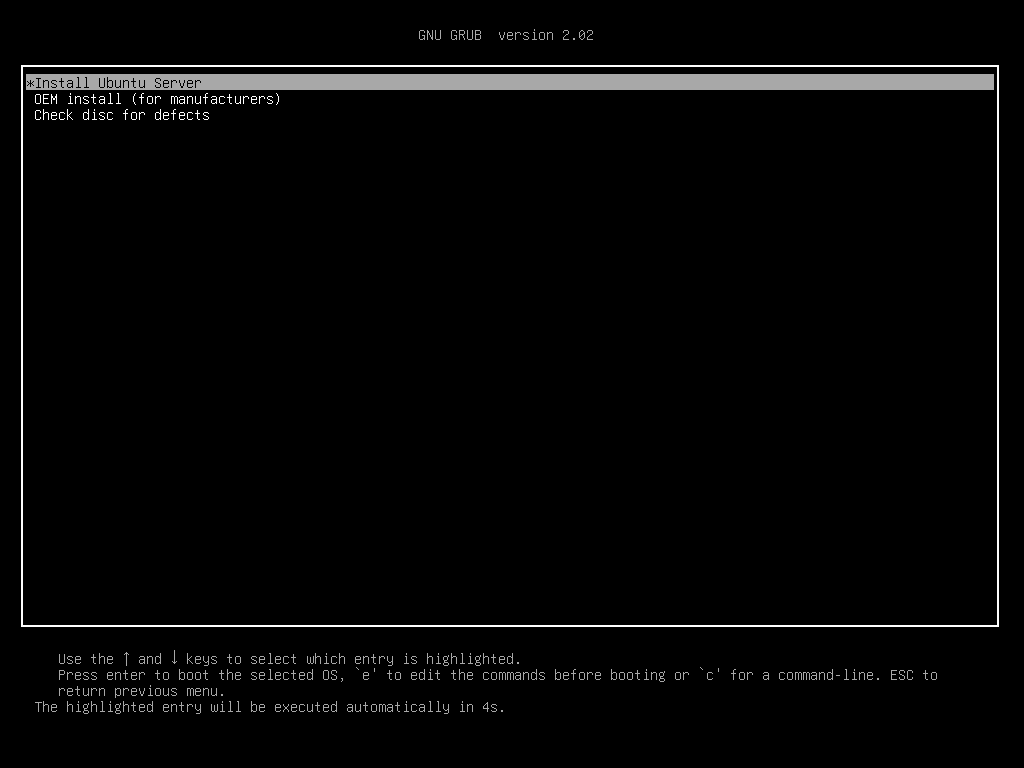
\includegraphics[width=1\textwidth]{screenshots/IY2D502-2019-02-21-19-15-19.png}
\caption{Selecting \texttt{Install Ubuntu Server} at the GRUB2 boot menu}
\label{fig:IY2D502-2019-02-21-19-15-19}
\end{figure}
\pagebreak
\begin{figure}[h!]
\centering
\captionsetup{skip=\skipfigurecaptionlen}
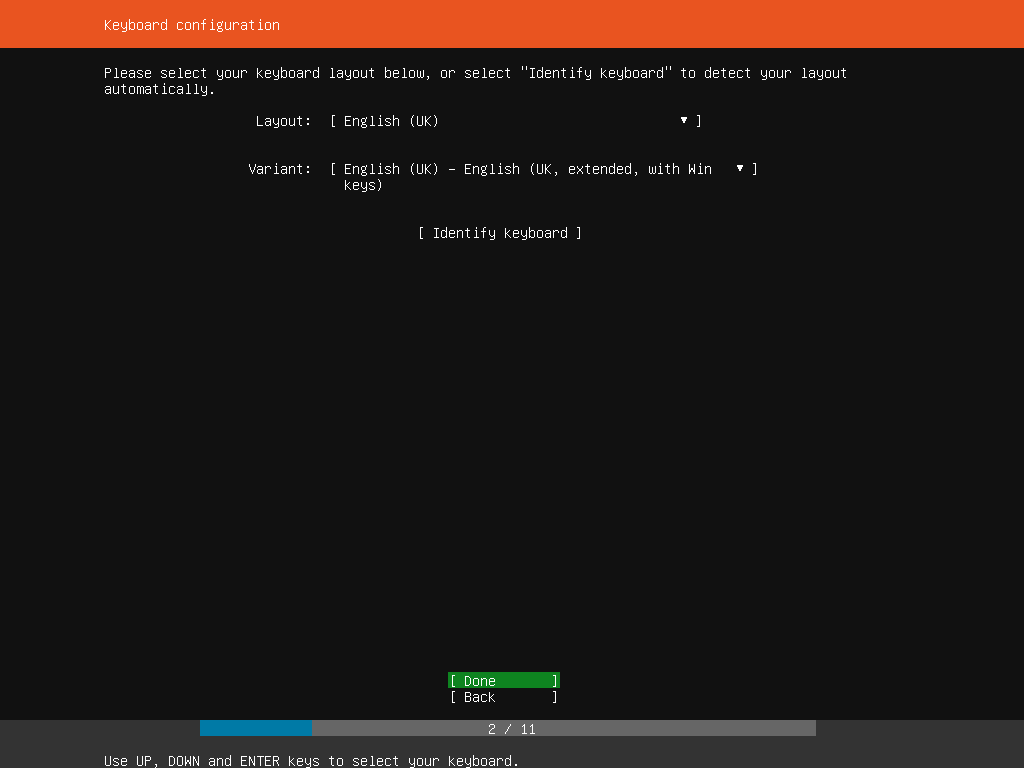
\includegraphics[width=1\textwidth]{screenshots/IY2D502-2019-02-21-19-16-03.png}
\caption{Configuring a sensible keyboard layout and variant for standard UK keyboards}
\label{fig:IY2D502-2019-02-21-19-16-03}
\end{figure}
\pagebreak
\begin{figure}[h!]
\centering
\captionsetup{skip=\skipfigurecaptionlen}
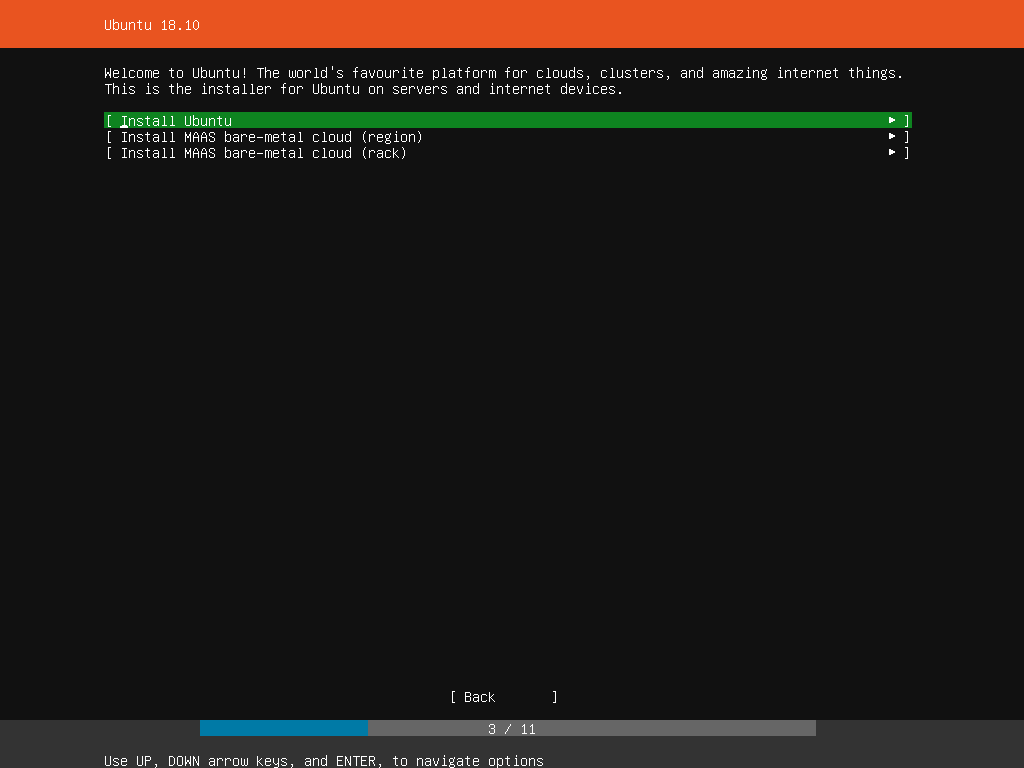
\includegraphics[width=1\textwidth]{screenshots/IY2D502-2019-02-21-19-16-06.png}
\caption{Selecting \texttt{Install Ubuntu} for a normal server deployment}
\label{fig:IY2D502-2019-02-21-19-16-06}
\end{figure}
\pagebreak
\begin{figure}[h!]
\centering
\captionsetup{skip=\skipfigurecaptionlen}
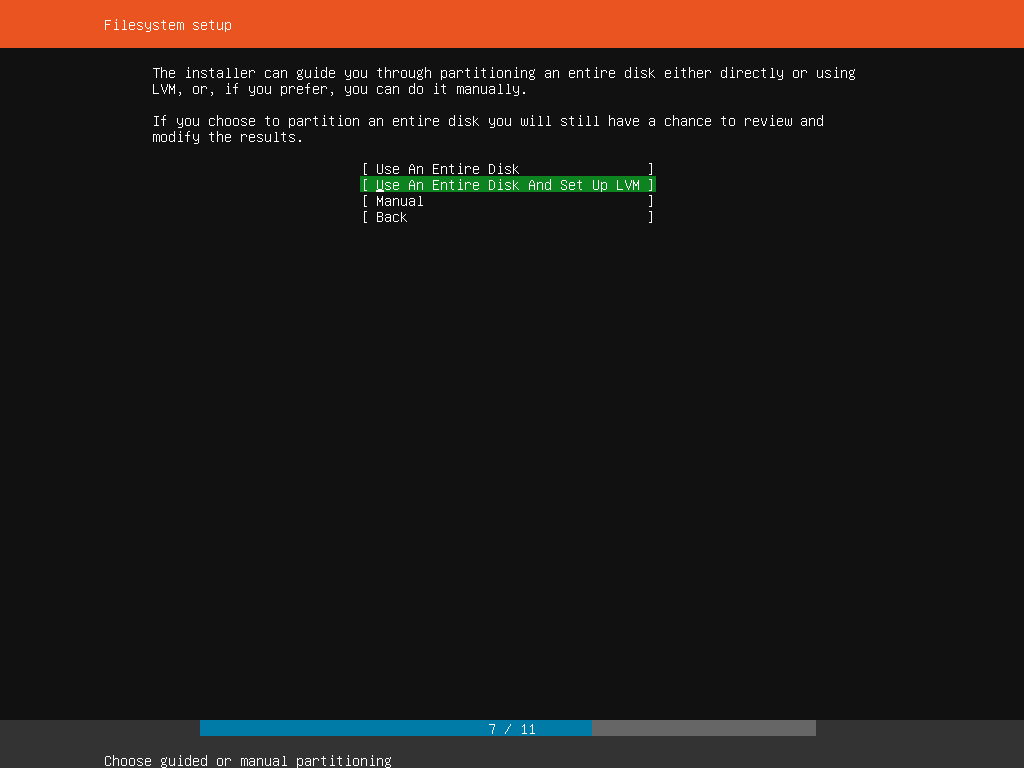
\includegraphics[width=1\textwidth]{screenshots/IY2D502-2019-02-21-19-16-38.png}
\caption{Choosing to use Logical Volume Management for filesystem partitioning}
\label{fig:IY2D502-2019-02-21-19-16-38}
\end{figure}
\pagebreak
\begin{figure}[h!]
\centering
\captionsetup{skip=\skipfigurecaptionlen}
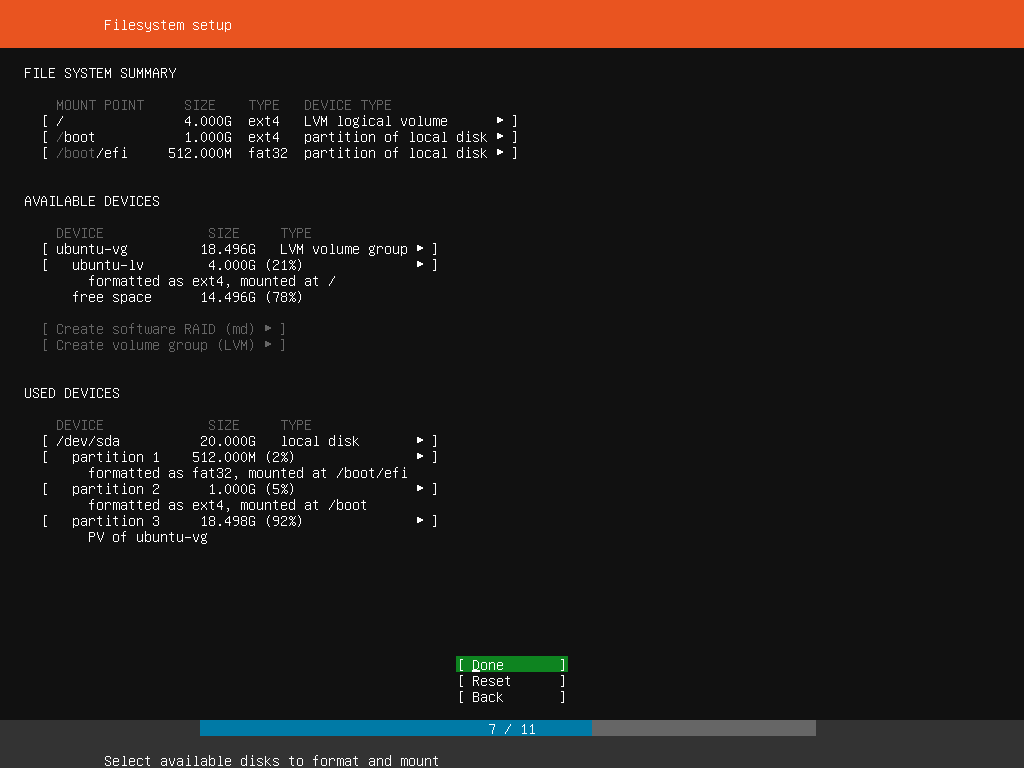
\includegraphics[width=1\textwidth]{screenshots/IY2D502-2019-02-21-19-16-43.png}
\caption{Confirming the default LVM configuration}
\label{fig:IY2D502-2019-02-21-19-16-43}
\end{figure}
\pagebreak
\begin{figure}[h!]
\centering
\captionsetup{skip=\skipfigurecaptionlen}
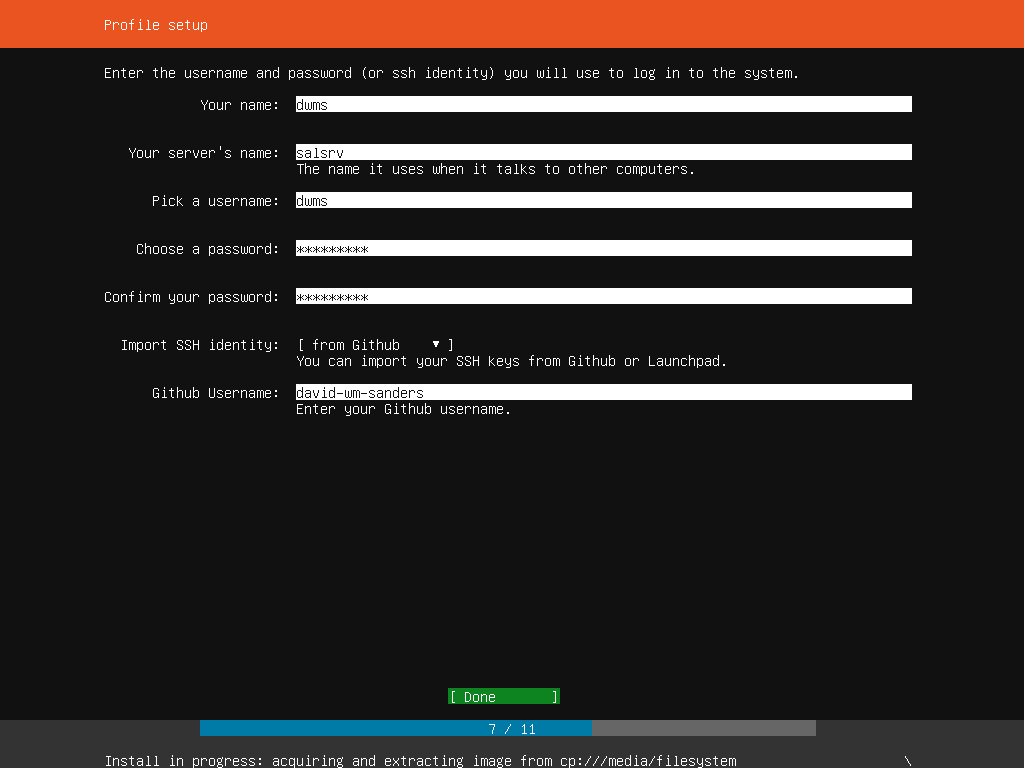
\includegraphics[width=1\textwidth]{screenshots/IY2D502-2019-02-21-19-17-27.png}
\caption{Configuring server and importing personal SSH identity from \faGithub\ GitHub}
\label{fig:IY2D502-2019-02-21-19-17-27}
\end{figure}
\pagebreak
\begin{figure}[h!]
\centering
\captionsetup{skip=\skipfigurecaptionlen}
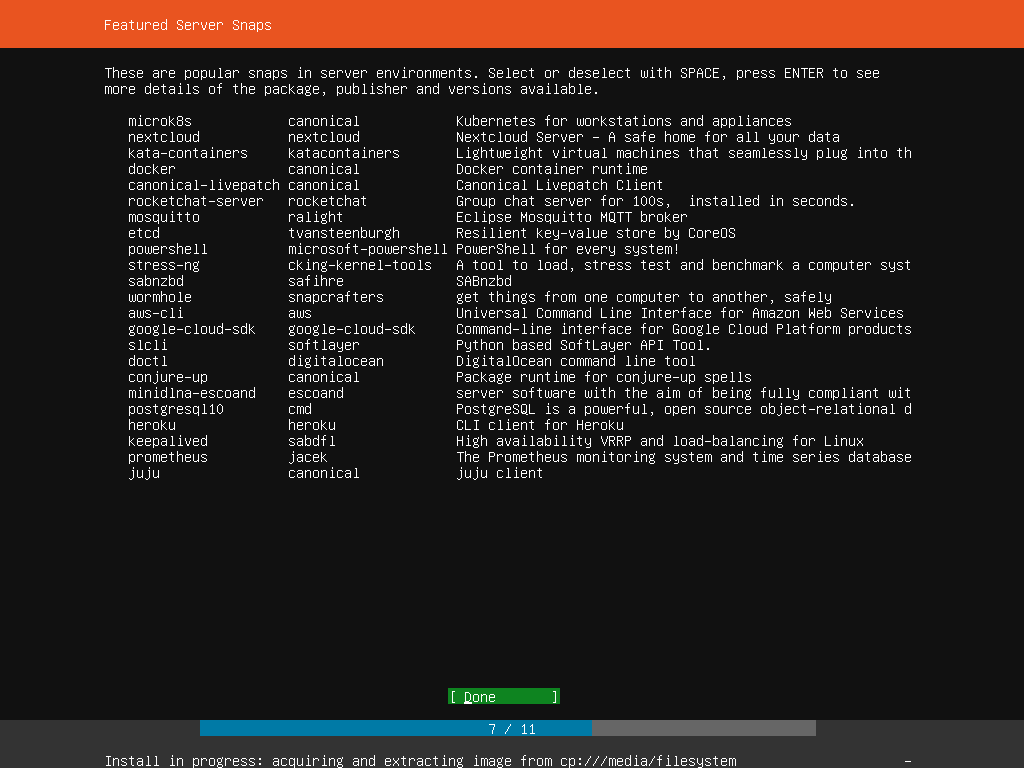
\includegraphics[width=1\textwidth]{screenshots/IY2D502-2019-02-21-19-17-58.png}
\caption{Reviewing snap configurations and deciding to install docker manually}
\label{fig:IY2D502-2019-02-21-19-17-58}
\end{figure}
\pagebreak
\begin{figure}[h!]
\centering
\captionsetup{skip=\skipfigurecaptionlen}
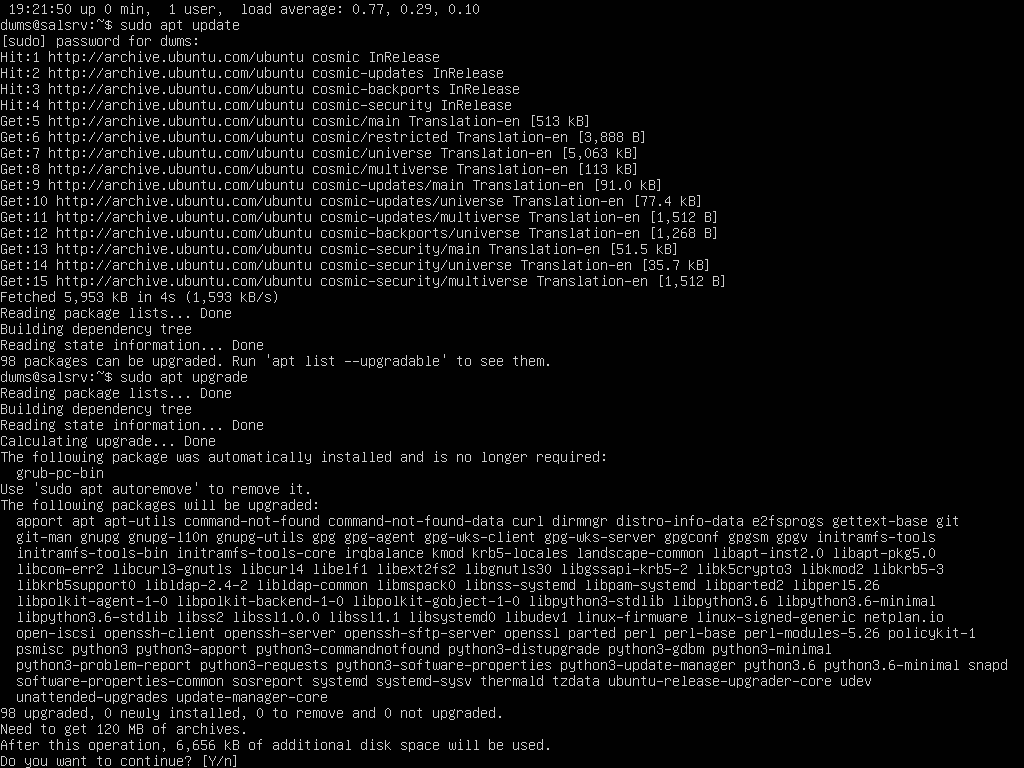
\includegraphics[width=1\textwidth]{screenshots/IY2D502-2019-02-21-19-22-44.png}
\caption{Upgrading the server immediately after first boot to get all security patches}
\label{fig:IY2D502-2019-02-21-19-22-44}
\end{figure}
\pagebreak
\begin{figure}[h!]
\centering
\captionsetup{skip=\skipfigurecaptionlen}
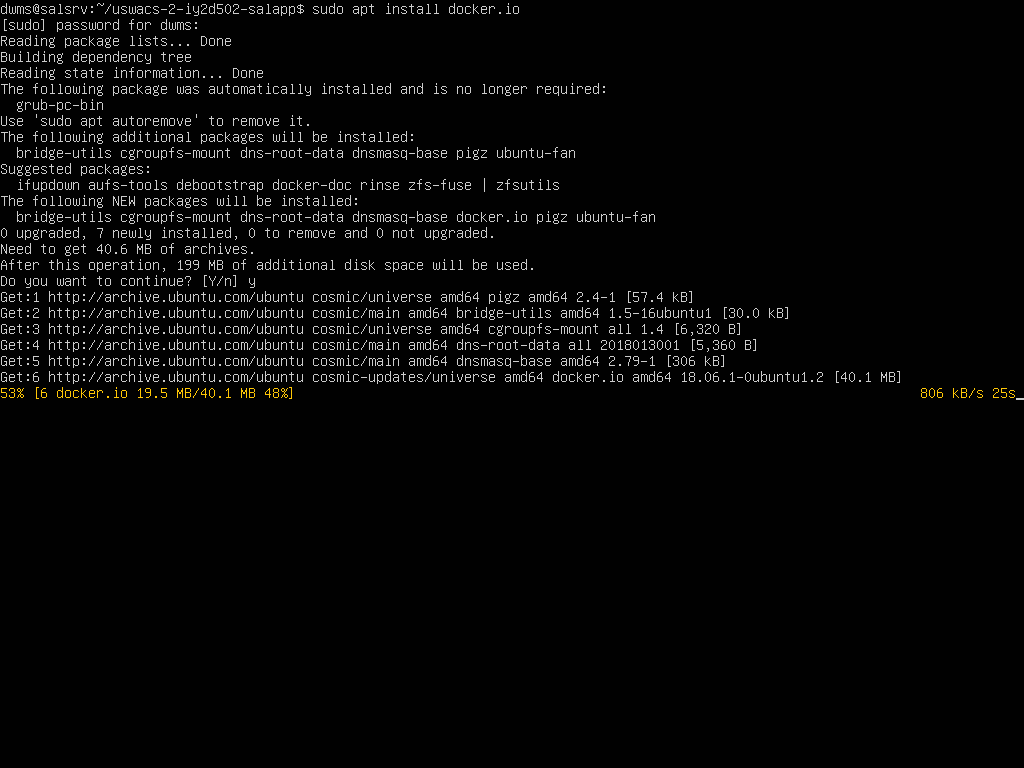
\includegraphics[width=1\textwidth]{screenshots/IY2D502-2019-02-21-23-29-41.png}
\caption{Installing \texttt{docker.io} using \texttt{apt install}}
\label{fig:IY2D502-2019-02-21-23-29-41}
\end{figure}
\pagebreak
\begin{figure}[h!]
\centering
\captionsetup{skip=\skipfigurecaptionlen}
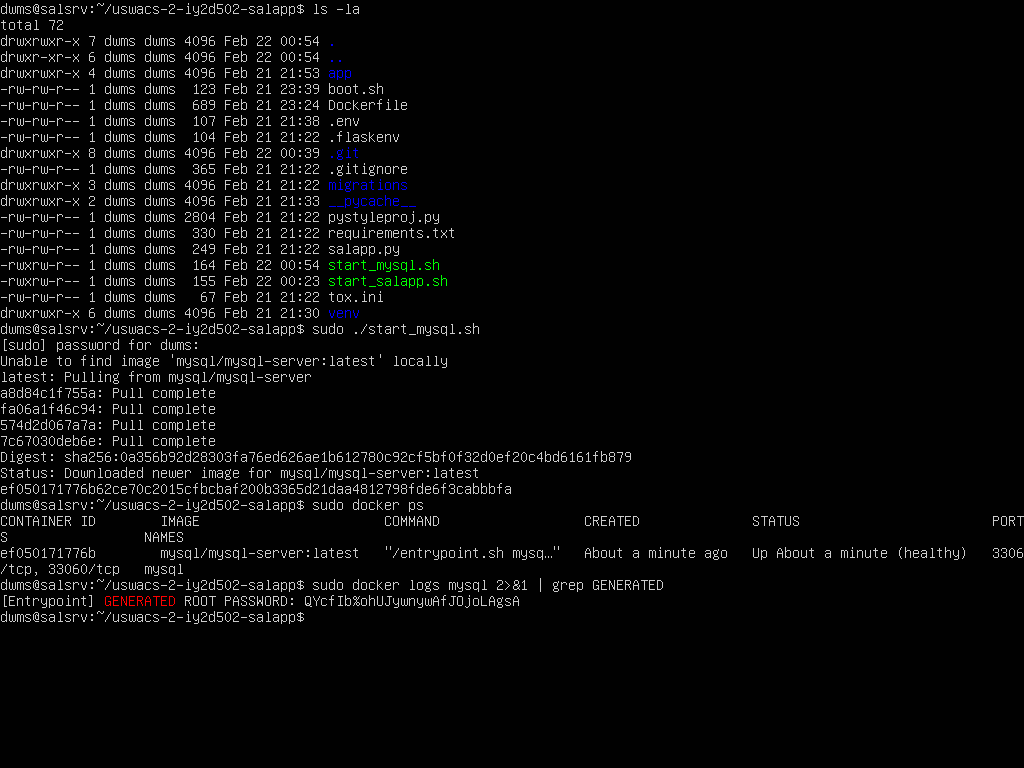
\includegraphics[width=1\textwidth]{screenshots/IY2D502-2019-02-22-00-58-41.png}
\caption{Starting up a MySQL instance in a docker container}
\label{fig:IY2D502-2019-02-22-00-58-41}
\end{figure}
\pagebreak
\begin{figure}[h!]
\centering
\captionsetup{skip=\skipfigurecaptionlen}
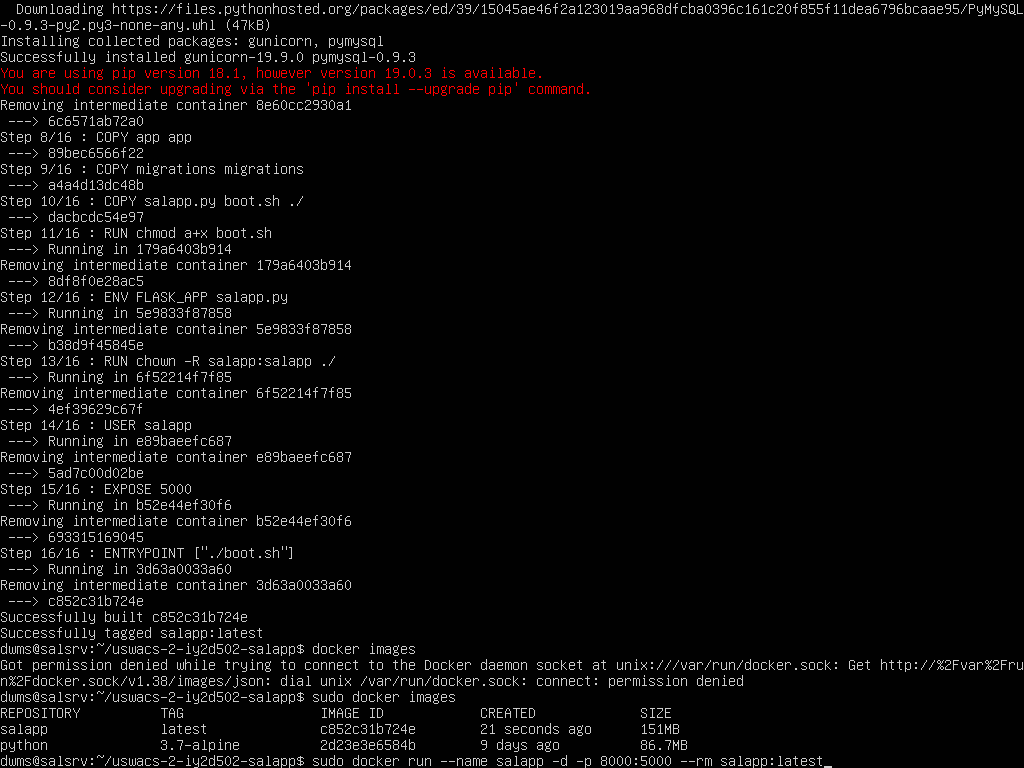
\includegraphics[width=1\textwidth]{screenshots/IY2D502-2019-02-21-23-43-07.png}
\caption{Building a custom docker image for \texttt{salapp}}
\label{fig:IY2D502-2019-02-21-23-43-07}
\end{figure}
\pagebreak
\begin{figure}[h!]
\centering
\captionsetup{skip=\skipfigurecaptionlen}
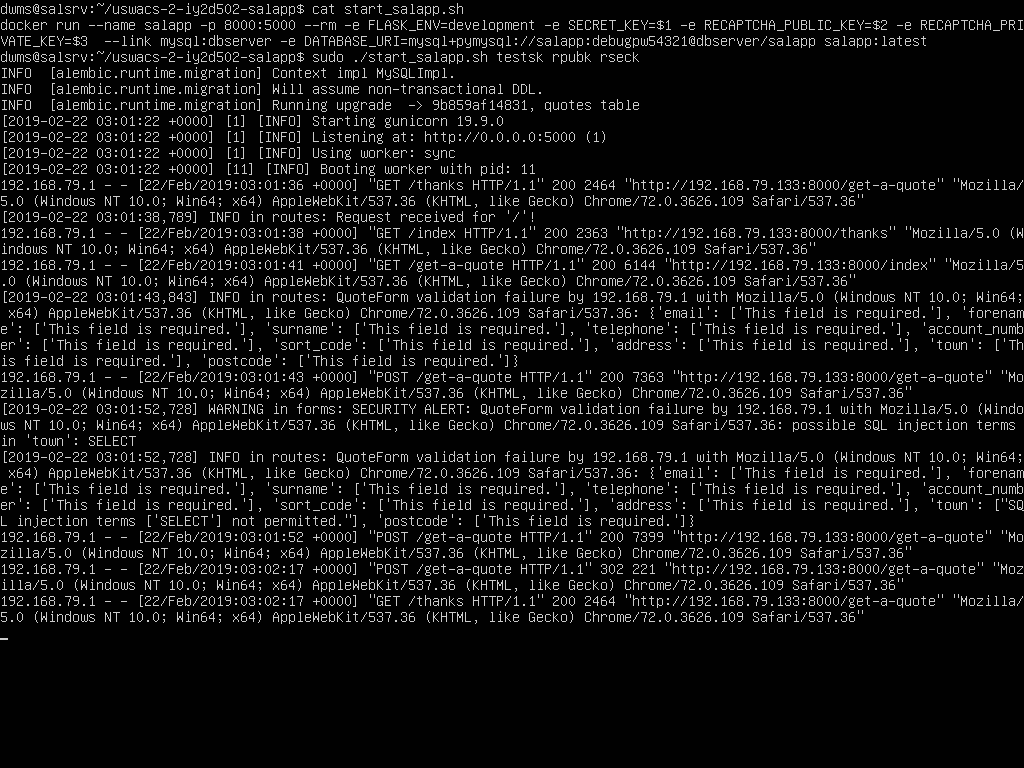
\includegraphics[width=1\textwidth]{screenshots/IY2D502-2019-02-22-03-02-25.png}
\caption{Starting up a non-detached \texttt{salapp} instance for testing}
\label{fig:IY2D502-2019-02-22-03-02-25}
\end{figure}

\pagebreak
\begin{figure}[h!]
\centering
\captionsetup{skip=\skipfigurecaptionlen}
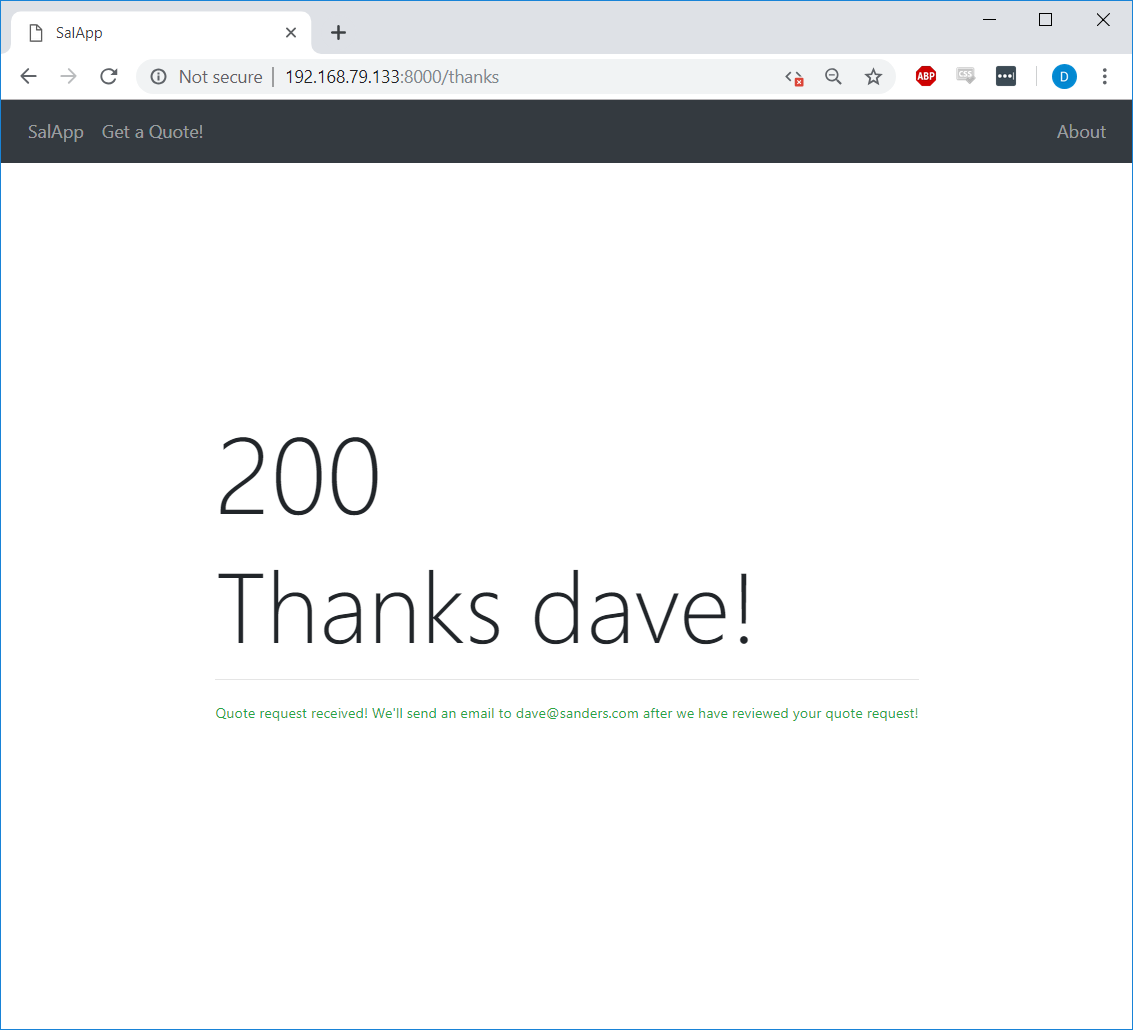
\includegraphics[width=1\textwidth]{screenshots/salapp1.png}
\caption{Providing quote data to the form that passes validation}
\label{fig:salapp1}
\end{figure}

\pagebreak
\begin{figure}[h!]
\centering
\captionsetup{skip=\skipfigurecaptionlen}
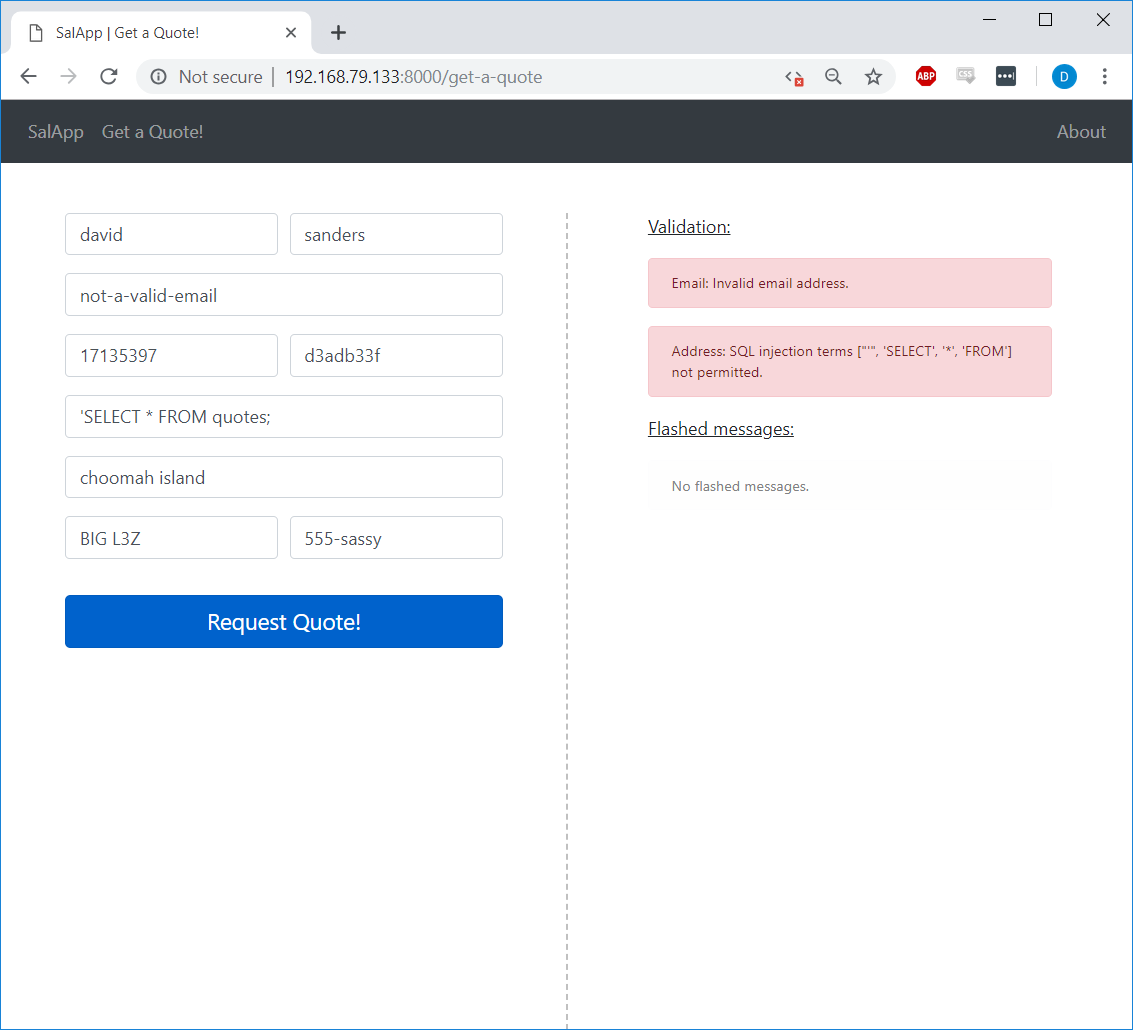
\includegraphics[width=1\textwidth]{screenshots/salapp2.png}
\caption{Providing quote data to the form that fails validation}
\label{fig:salapp2}
\end{figure}

\pagebreak
\begin{figure}[h!]
\centering
\captionsetup{skip=\skipfigurecaptionlen}
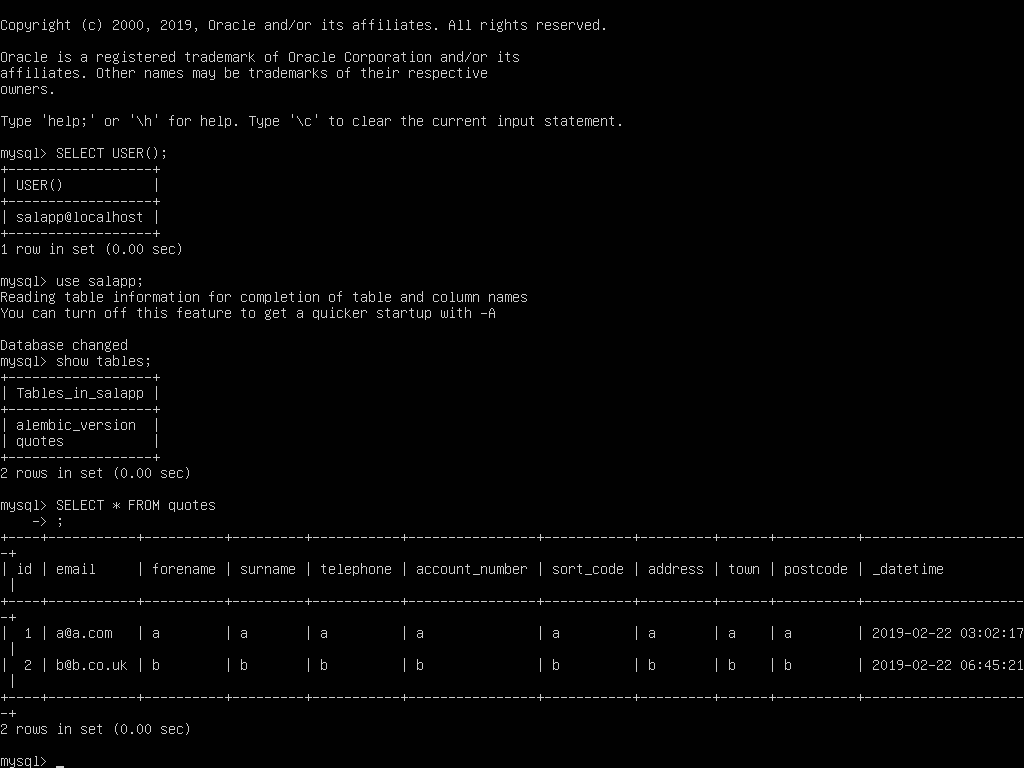
\includegraphics[width=1\textwidth]{screenshots/IY2D502-2019-02-22-06-50-24.png}
\caption{Checking that successfully validated quotes were inserted into the database}
\label{fig:IY2D502-2019-02-22-06-50-24}
\end{figure}

\pagebreak
\begin{figure}[h!]
\centering
\captionsetup{skip=\skipfigurecaptionlen}
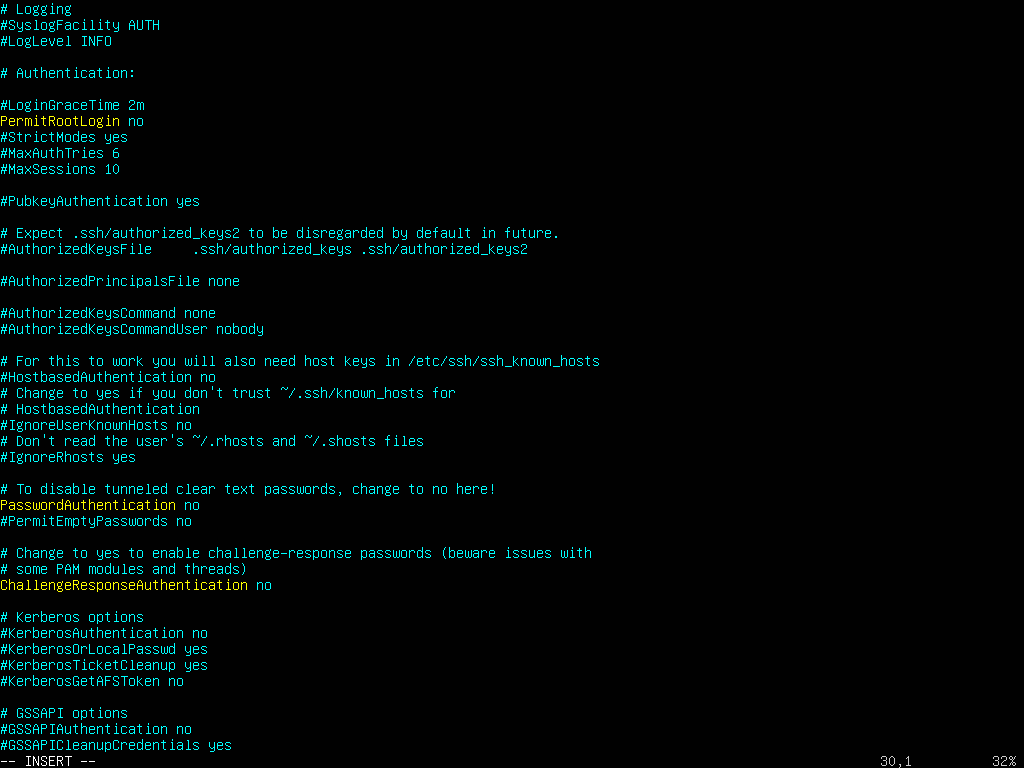
\includegraphics[width=1\textwidth]{screenshots/IY2D502-2019-02-26-17-44-30.png}
\caption{Hardening the SSH server configuration in \texttt{vim}}
\label{fig:IY2D502-2019-02-26-17-44-30}
\end{figure}

% \pagebreak
% \begin{figure}[h!]
% \centering
% \captionsetup{skip=\skipfigurecaptionlen}
% 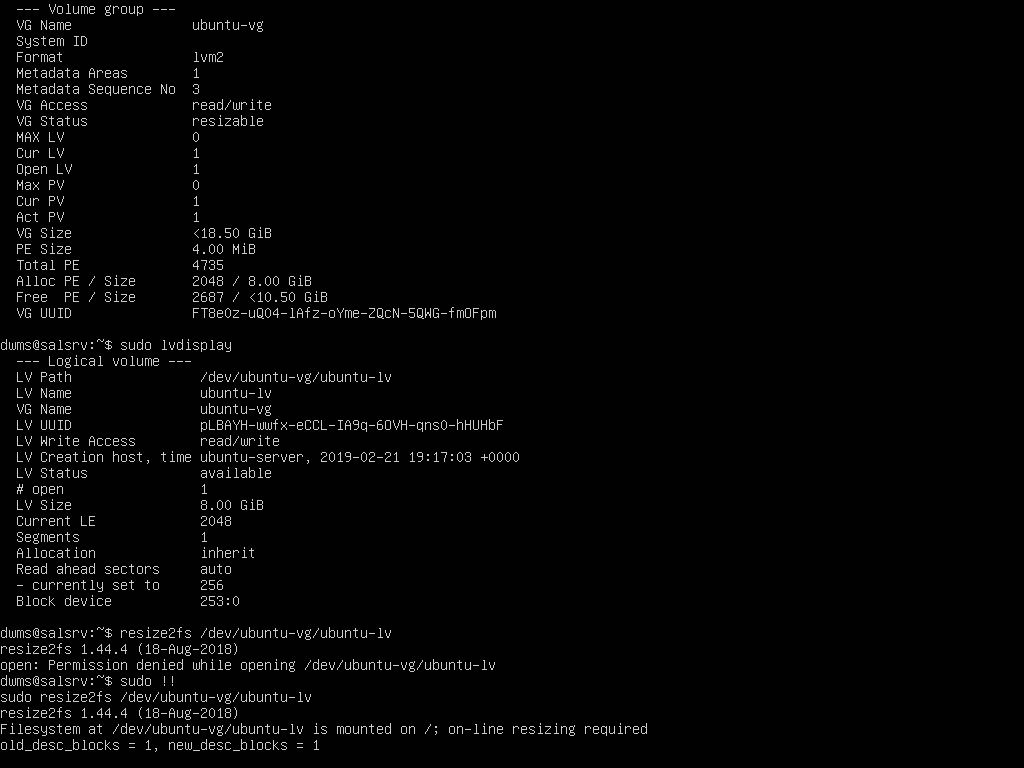
\includegraphics[width=1\textwidth]{screenshots/IY2D502-2019-02-22-23-39-52.png}
% \caption{Resizing the \texttt{/} logical volume}
% \label{fig:IY2D502-2019-02-22-23-39-52}
% \end{figure}
% \pagebreak
% \begin{figure}[h!]
% \centering
% \captionsetup{skip=\skipfigurecaptionlen}
% 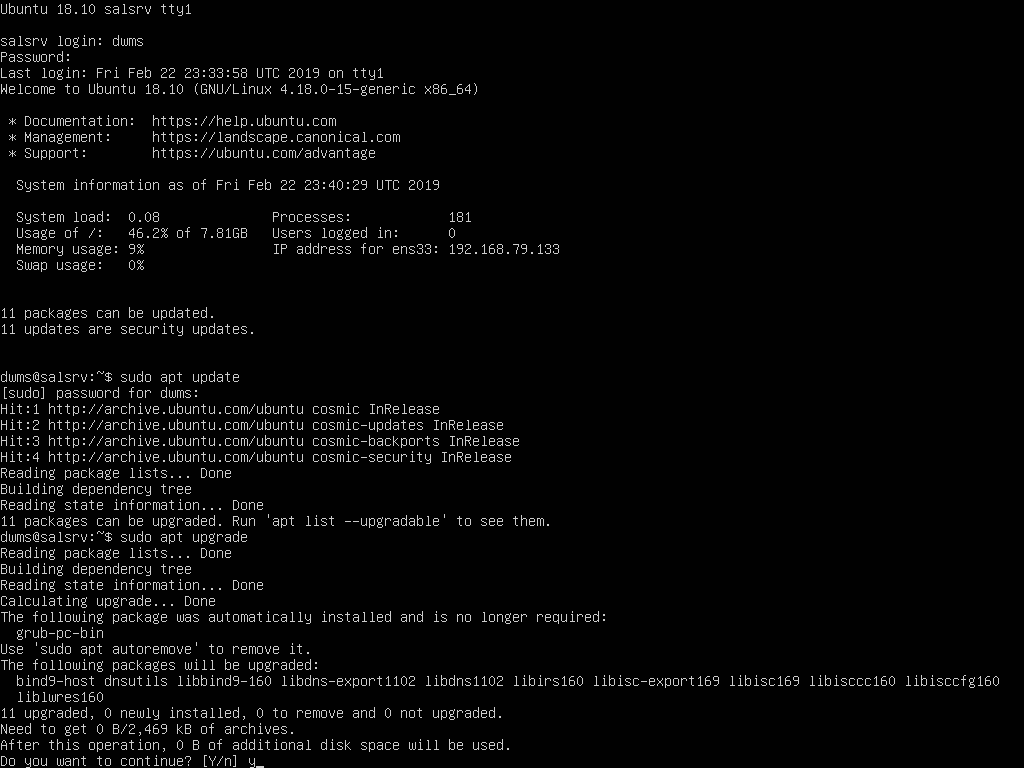
\includegraphics[width=1\textwidth]{screenshots/IY2D502-2019-02-22-23-41-29.png}
% \caption{Noticing that there are security updates on reboot and upgrading immediately}
% \label{fig:IY2D502-2019-02-22-23-41-29}
% \end{figure}
% \pagebreak
% \begin{figure}[h!]
% \centering
% \captionsetup{skip=\skipfigurecaptionlen}
% 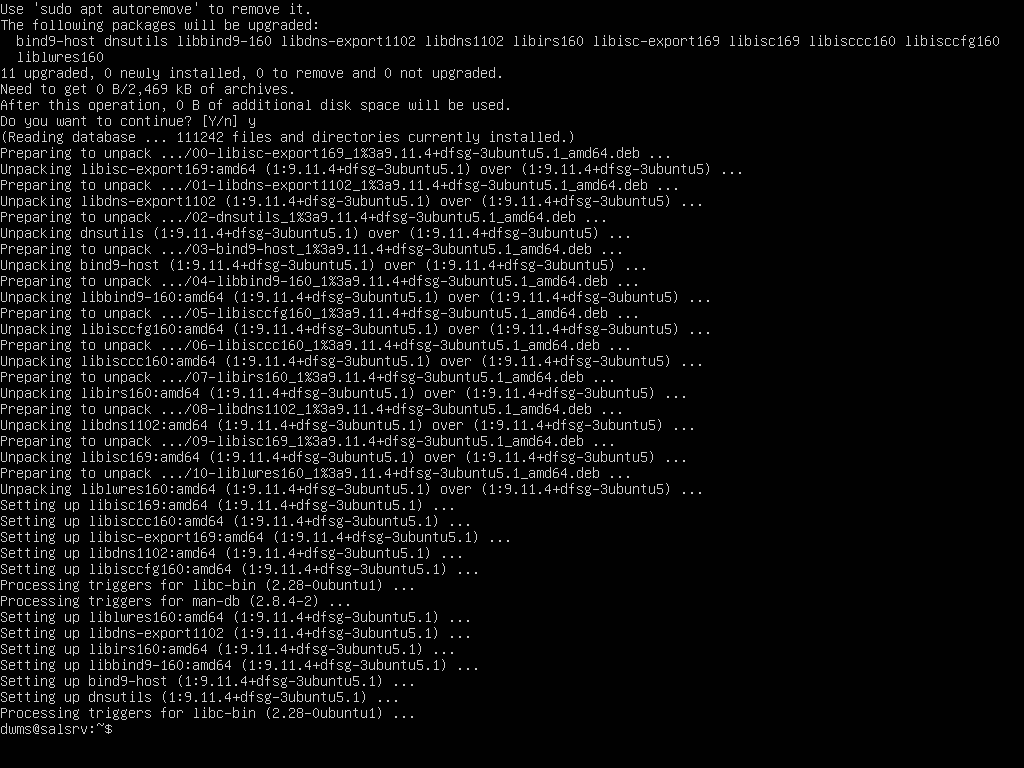
\includegraphics[width=1\textwidth]{screenshots/IY2D502-2019-02-22-23-44-52.png}
% \caption{Upgrading packages to fix security issues in \texttt{bind9} and others}
% \label{fig:IY2D502-2019-02-22-23-44-52}
% \end{figure}
% \pagebreak
% \begin{figure}[h!]
% \centering
% \captionsetup{skip=\skipfigurecaptionlen}
% 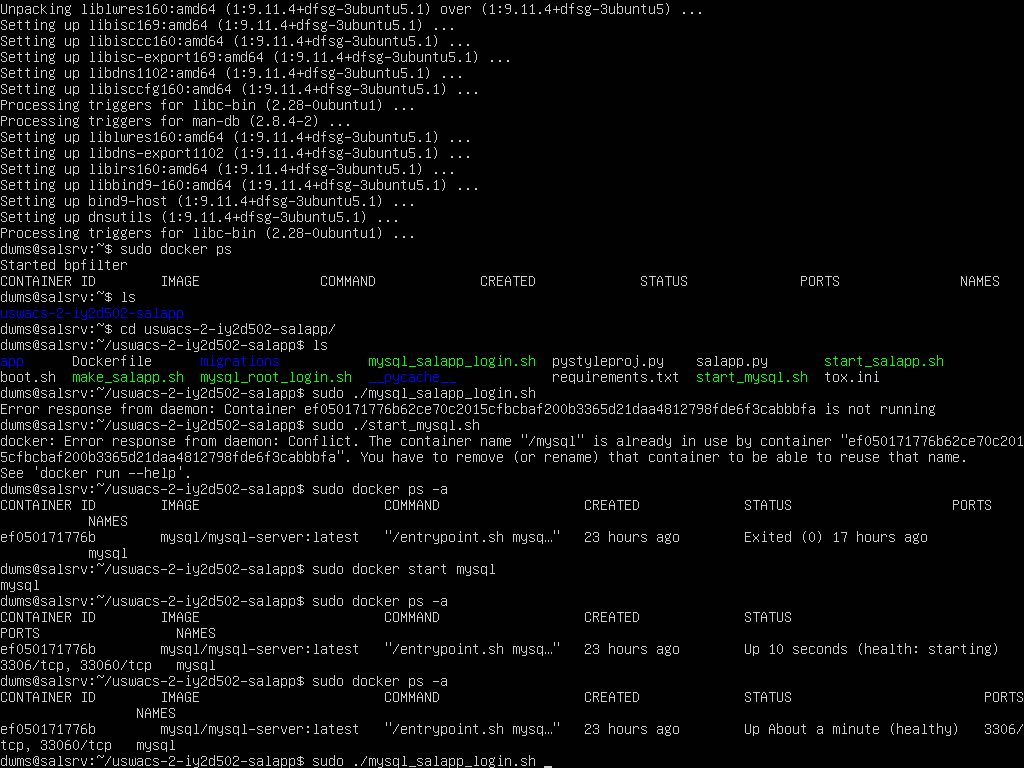
\includegraphics[width=1\textwidth]{screenshots/IY2D502-2019-02-22-23-49-29.png}
% \caption{Restarting the MySQL container after reboot and waiting for \texttt{healthy} status}
% \label{fig:IY2D502-2019-02-22-23-49-29}
% \end{figure}
\pagebreak
\begin{figure}[h!]
\centering
\captionsetup{skip=\skipfigurecaptionlen}
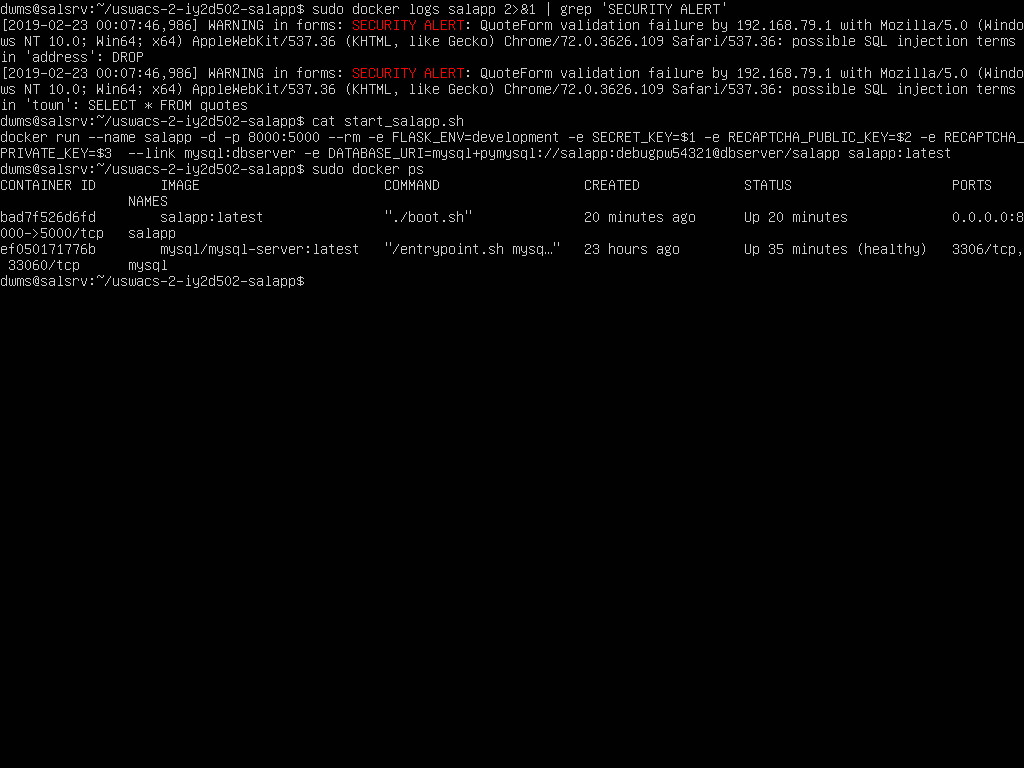
\includegraphics[width=1\textwidth]{screenshots/IY2D502-2019-02-23-00-23-12.png}
\caption{Checking logs from the running salapp container for security alert messages}
\label{fig:IY2D502-2019-02-23-00-23-12}
\end{figure}
\pagebreak


\end{document}
